\Huge\textbf{Capitolo 7: \\Proteine di membrana destinate a organelli differenti}\\

\small
In generale, la conformazione di una proteina influisce sulla sua destinazione, quindi si basa sulla composizione AA. In un preciso stratch di AA si racchiude la chiave per il target (solitamente all'N terminale), ogni organello ha recettori specifici per la propria sequenza terminale e dei traslocatori per la destinazione. 
Talvolta la targeting sequence è rimossa, ha \textbf{determinata natura chimicha, specifici recettori, specifici canali traslocatori e consuma una determinata fonte di energia.}

\section{Regolazione delle proteine}
    A prescindere dal compartimento cellulare, le proteine possono essere modificate chimicamente per ottenere un comportamento differente. 
    \subsection{Fosforilazione}
        Per fosforilazione di intende l'aggiunta di un gruppo fosfato alla proteina target in corrispondenza di un gruppo ossidrile, tramite una reazione di condensazione. Generalmente sono serina, tisorina e treonina che subiscono questa modifica. \\
        Può avvenire in qualunque compartimento cellulare.
        
    \subsection{Allosteria}
        Per allosteria si intende l'utilizzo di un ligando allosterico che si associa alla proteina in un particolare sito. Questo determina un cambiamento conformazionale di un sito A che determina l'attivazione di un sito B.\\
        Esempi di questa modalità di attivazione sono la Calmodulina tramite lo ione $Ca^{++}$ oppure RAN assieme a GTP e GDP.
        
    \subsection{Ubiquitinazione}
        Per ubiquitinazione si intende l'associazione di ubiquitina (UB) (generalmente catene) per la regolazione dell'emivita della proteina target. Il legame con la catena di ubiquitine determina l'associazione con il proteasoma. \\
        L'UB è una piccola molecola proteica (di soli 76 AA di cui 7 lisine) che risulta estremamente conservata tra speci differenti. Viene utilizzata come marker per la morte di una molecola proteica.\\
            
        L'ubiquitinazione avviene attraverso l'utilizzo di diversi enzimi:
        \begin{enumerate}
            \item E1 (enzima di attivazione dell'UB) che si associa covalentemente a una cisteina dell'UB
            \item E2 (enzima per la coniugazione dell'UB) che forma un legame covalente con una cisteina dell'UB (funzione simile ad E1)
            \item E3 (enzima ligasi per l'UB) che viene promossa dalla presenza di E2 che predispone il substrato proteico per il legame tra esso e l'UB
            \item E4 (non essenziale) che allunga le catene di UB pre-esistenti.
        \end{enumerate}
        Esistono 2 geni per E1, 35 per E2 e più di 100 per E3, questo per aumentare la specificità a substrati diversi. In particolare esistono HECT e RING (due tipologie di E3) che sostengono rispettivamente un legame covalente o un trasferimento diretto. \\
        
        La poliubiquitinazione ha come scopo l'associazione al proteasoma, una macromolecola in grado di degradare la proteina in monomeri o dimeri di AA. Il proteasoma ha dei recettori per UB (lega catene di UB), contiene DUB (de-ubiquitinazione, dissociazione da UB), AAA-ATPasi per svolgere il polipeptide da degradare.\\
        L'aggiunta di UB può avvenire in maniere diverse che assumono scopi differenti, ubiquitinazioni differenti dalla proteina hanno funzioni tuttora ignote e possibilmente molto differenti:
        \begin{itemize}
            \item Poli-UB: segnala la morte della proteina e l'intervento del proteasoma
            \item Multi-UB: UB non forma una catena ma è associata a siti differenti
            \item Mono-UB
            \item Poli-UB ramificate: formazione di ramificazioni di UB tramite legami isopeptidici tra il C-terminale di un UB e una catena laterale di un'altra UB che funge da substrato.\\
            A seconda della lisina coinvolta nell'UB (sono 7 in totale) del substrato assume comportamenti differenti: 
                \begin{itemize}
                    \item Lisina 48: degradazione con proteasoma
                    \item Lisina 63: signaling immunitario
                    \item Lisina 33: controllo linfociti
                    \item Lisina 11: divisione cellulare
                \end{itemize}
        \end{itemize}

\section{Destinazione: RE}
    La sintesi proteica avviene al livello di citoplasma, possibilmente attraverso i ribosomi associati alla membrana del RE. 
    Dopo un'adeguata procedura, si riescono ad ottenere sperimentalmente i mircosomi, ovvero delle vescicole originate dal RE con ribosomi associati utili al fine di studi specifici.
    
    \subsection{Sequenza di targeting}
            Le sequenze di targeting (TS) sono specifiche sequenze di 16-30 AA poste all'N-terminale. Contiene sempre 1 o 2 AA carichi positivamente adiacenti ad uno stretch idrofobico di 6-12 AA. Gli AA idrofobici sono essenziali per la sequenza di targeting.
            Solitamente viene rimossa una volta che la proteina raggiunge il lumen. \\
            Effettuando un esperimento con dei microsomi, si osserva che l'importazione della proteina nel lumen avviene co-traduzionalmente, in particolare la traslocazione avviene entro la traduzione dei primi 70 AA. La TS è compresa nei primi 40 AA quindi risulta già esposta alle proteine traslocanti.\\
            
            \subsubsection{SRP}
                La SRP (\textit{signal recognition particle}) è una ribonucleoproteina che è composta di 6 polipeptidi e un RNA di circa 300 nucleotidi. P54, uno degli esameri che la compongono, interagisce con le TS grazie al suo canale che favorisce l'associazione con la porzione idrofobica.\\
                Un dominio differente lega invece un GTP che promuove l'associazione con un recettore di SRP, una proteina integrale di membrana presente sulla porzione citosolica.
            
            \subsubsection{Importazione}
                \begin{enumerate}
                    \item Il ribosoma sintetizza la prima porzione proteica
                    \item SRP allaccia la porzione idrofobica di TS e la stabilizza
                    \item SRP stabilisce interazioni con i recettori SRP nel momento in cui entrambi sono legati a GTP (specificità)
                    \item avviene l'idrolisi del GTP promossa su entrambi nel momento in cui il complesso è ormai formato che determina l'apertura del canale proteico (il traslocone).
                    \item la TS viene associata al traslocone e avviene il rilascio di SRP
                    \item il neo-polipeptide viene sintetizzato attivamente e grazie all'aumento di AA viene spinto attraverso il traslocone
                    \item la TS viene rimossa
                    \item nel momento il cui il ribosoma incontra il codone di stop si ferma la polimerizzazione, viene rilasciato il traslocone e avviene il rilascio della proteina.
                \end{enumerate}
                \begin{figure}[h]
                    \centering
                    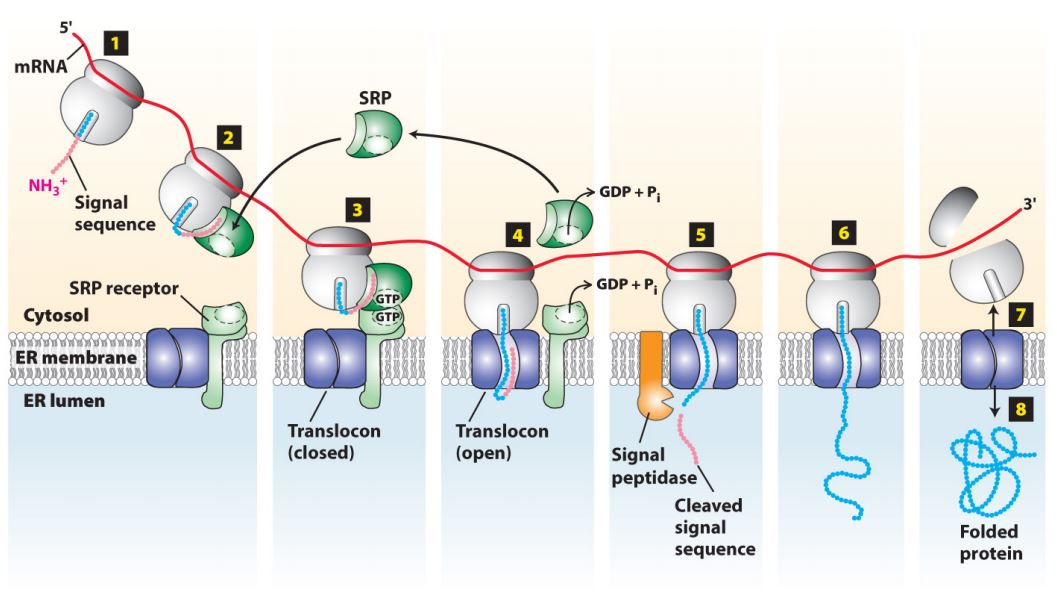
\includegraphics[width=0.7\textwidth]{images/importazioneRE.JPG}
                    \caption{\small Step dell'importazione di una proteina che presenta TS nel RE}
                    \label{fig:mesh1}
                \end{figure}
        
    \subsection{Trasloconi e canali}
        Il traslocone dedito al passaggio dei polipeptidi citato sopra è chiamato SEC61$\alpha$. Presenta una struttura a forma di poro "ristretto" con $\alpha$E di leucina che entrano a contatto con il polipeptide da traslocare.
        Assume la capacità di dilatarsi nel momento in cui viene a contatto con il polipeptide (gating, è presente una componente "plug" che libera ed ostruisce il canale). \\
        SEC63 insieme a SEC61$\alpha$ è un altro meccanismo di traslocazione ma avviene a livello post-traduzionale. Non vi è il coinvolgimento di SRP.
        Viene sostenuto da componenti accessorie che promuovono l'associazione di particoalri proteine (BiP, una chaperon) che lega e idrolizza ATP e in seguito cambia conformazione e diventa prono a legare un polipeptide.  \\
        Risulta quindi possibile traslocare porzioni proteiche a livello post-traduzionale, il principio di funzionamento è molto differente: non è l'energia dell'ATP della traduzione a promuovere la traslocazione, ma sono molteplici molecole di BiP che associate ad una sistematica idrolisi favoriscono l'import dal punto di vista energetico. 
        Una volta traslocata BiP si dissocia e la proteina può assumere la sua conformazione.
        \begin{figure}[h]
            \centering
            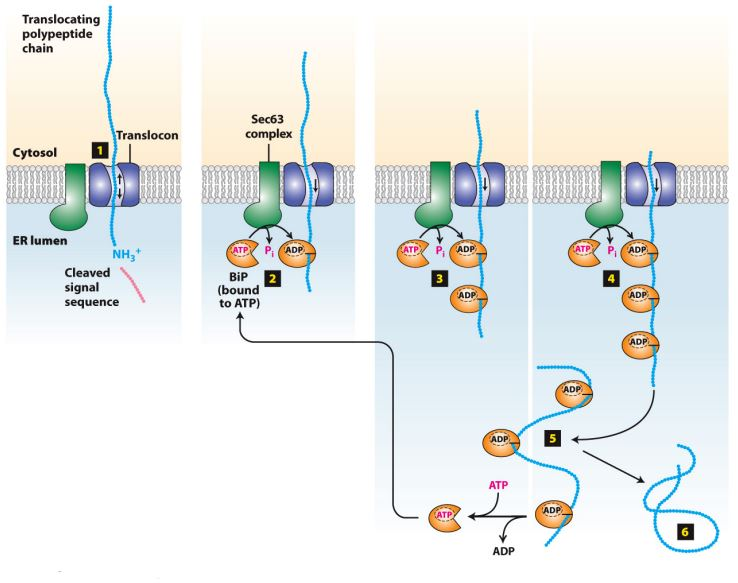
\includegraphics[width=0.7\textwidth]{images/importazioneSEC63-61.JPG}
            \caption{\small Step dell'importazione di una proteina a livello post-traduzionale grazie a SEC61 e SEC63}
            \label{fig:mesh1}
        \end{figure}
        
    \subsection{Sequenze di targeting e inserimento}
        Esistono molte tipologie di proteine transmembrana che dipendono dalle loro sequenze topogeniche, dalla loro posizione e dal loro orientamento. 
        \subsubsection{Sequenze topogeniche}
            \begin{itemize}
                \item \textbf{TS} all'N-terminale
                \item \textbf{STA}, stop transfer anchor interna alla sequenza
                \item \textbf{SA}, anchor signal, simile alla sequenza TS, presenta allo stesso modo una porzione di AA in prossimità dello stretch idrofobico ma è interna alla sequenza AA
            \end{itemize}
            Di seguito le tipologie di proteine transmembrana in base alle loro sequenze topogeniche.
        
        \subsubsection{Tipo 1}
            \begin{figure}[h]
                \centering
                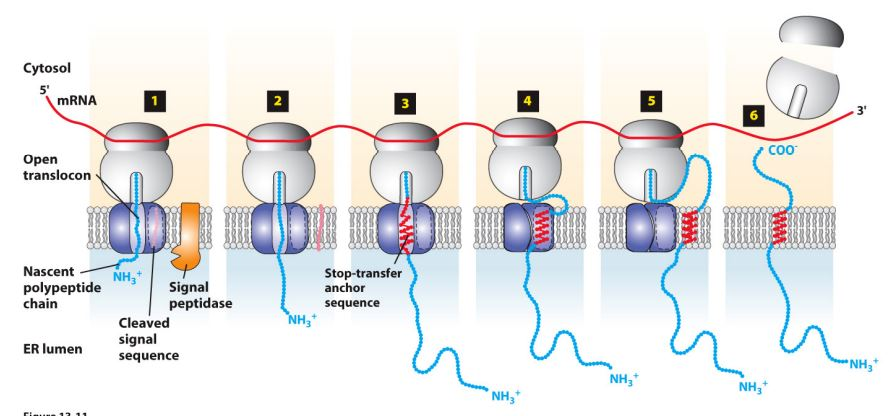
\includegraphics[width=0.7\textwidth]{images/Tipo1.JPG}
                \caption{\small Ancoraggio alla membrana delle proteine di tipo 1}
                \label{fig:mesh1}
            \end{figure}
            Sono polipeptidi con una sequenza topogenica di tipo TS e una STA.\\
            Sono composte da una singola $\alpha$E transmembrana. \\
            \begin{enumerate}
                \item La traduzione inizia da TS all'N-terminale
                \item Produzione di uno stretch altamente idrofobico.
                \item Traduzione della STA
                \item STA raggiunge il traslocone che cambia conformazione in corrispondenza con STA e lascia diffondere lateralmente l'ancora proteica nella membrana
                \item il ribosoma rimane associato fino al codone di stop e poi si dissocia
            \end{enumerate}
            
        \subsubsection{Tipo 2 e 3}
            \begin{figure}[h]
                \centering
                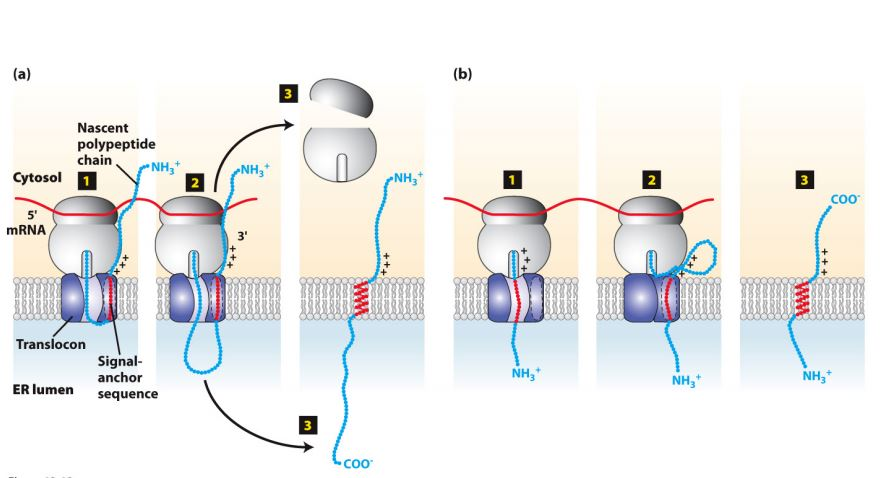
\includegraphics[width=0.7\textwidth]{images/Tipo23.JPG}
                \caption{\small Ancoraggio alla membrana delle proteine di tipo 2 e 3}
                \label{fig:mesh1}
            \end{figure}
            Sono polipeptidi con un singolo SA. \\
            Sono composte da una singola $\alpha$E transmembrana. 
            \begin{enumerate}
                \item Inizio della traduzione della proteina, compresa la porzione contenente AS
                \item SRP riconosce SA e inizia la traslocazione a valle
                \item il ribosoma incontra il codone di stop e si dissocia
            \end{enumerate}
            La differenza tra tipo 2 e tipo 3 sta nella posizione della porzione di AA positivi in relazione allo stretch SA. Per una proteina di tipo 2 sono presenti gli AA positivi precedenti a AS, per quelle di tipo 3 sono posti successivamente.
            Questa piccola differenza fa sì che le proteine di tipo 2 rivolgano il proprio N-terminale a livello del citosol mentre quelle di tipo 3 rivolgano il proprio C-terminale sul lumen.
        
        \subsubsection{Tail Anchor Protein}
            \begin{figure}[h]
                \centering
                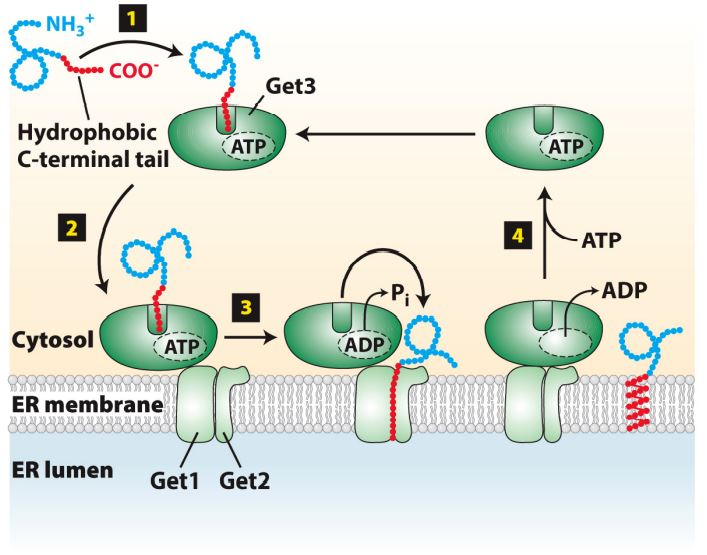
\includegraphics[width=0.5\textwidth]{images/TailAnchrProt.JPG}
                \caption{\small Ancoraggio alla membrana delle proteine di tipo tail anchor protein}
                \label{fig:mesh1}
            \end{figure}
            Sono polipeptidi contenenti una STA.\\
            Sono composte da una singola $\alpha$E transmembrana ma non hanno porzioni che si espongono sul lumen o sulla porzione esoplasmatica.\\
            Non sono coinvolti nè SRP nè il suo recettore, nè il traslocone.
            \begin{enumerate}
                \item La STA è posta al C-terminale, quindi la proteina è ormai interamente tradotta nel momento in cui appare STA
                \item STA viene riconosciuta da Get3 (presente nel citosol) che la protegge finchè non avviene l'interazione con Get1 e Get2
                \item Associazione con Get1 e Get2, idrolisi
                \item Passaggio per un traslocone dedicato
                \item apertura laterale del traslocone e inserimento STA nella membrana.
            \end{enumerate}
            
        \subsubsection{Tipo 4: multipass}
            Sono polipeptidi composti da diverse combinazioni delle classi precedenti. Sono presenti più stretch transmembrana e è possibile qualunque combinazione di N-terminali o C-terminali esposti sul lumen o sul citosol.\\
            Si possono distinguere le classi A e B (vedi figura).
            
        \subsubsection{GPI Anchor Protein}
            Sono polipeptidi contenenti una TS e una STA.\\
            Si associano ad un'ancora lipidica (GPI, \textit{glicosil fosfatidil inositolo}, un lipide con due catene idrofobe e una testa polare), hanno un dominio globulare al C-terminale a livello del lumen-esoplasmatico.
            \begin{enumerate}
                \item GPI è pre-esistente ed è già ancorato alla membrana.
                \item La proteina viene tradotta e traslocata come avviene per quelle di tipo 1. La traduzione viene ultimata prima del contatto con il GPI
                \item la proteina si associa al lipide attraverso l'enzima transamidasi (una sequenza di AA in prossimità a STA viene riconosciuta)
                \item STA rimane come prodotto di scarto
            \end{enumerate}
            Questa tipologia di proteine risulta dispendiosa a livello energetico. \\
            Vengono tuttavia sintetizzate perchè consente alle proteine di membrana di diffondere molto più rapidamente (grazie alla componente lipidica ancorata ad un singolo strato). In cellule con epiteli polarizzati, questa tipologia di ancora rappresenta un segnale per confinare una proteina ad un determinato dominio di membrana.
            \begin{figure}[h]
                \centering
                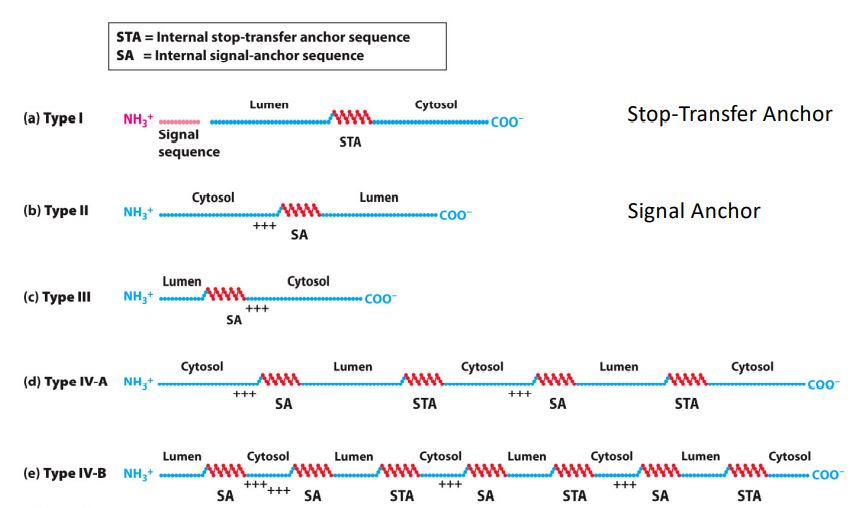
\includegraphics[width=0.7\textwidth]{images/sequenzeTopogeniche.JPG}
                \caption{\small Differenze dello stretch AA delle varie classi di proteine associate alla membrana}
                \label{fig:mesh1}
            \end{figure}
\pagebreak
            
\section{Destinazione: Nucleo}
    Le proteine che hanno accesso al nucleo sono già conformate tridimensionalmente. Passano attraverso il poro nucleare, che è il punto di discontinuità tra le due membrane nucleari quindi il punto di accesso.
    \subsection{Poro nucleare}
        Il poro nucleare (\textit{nuclear pore complex, NPC}) è un conglomerato proteico (16 volte più grande del ribosoma) formato da 30 polipeptidi differenti, le nucleoporine (NAP), ognuno dei quali presente in più copie.\\
        Il NPC è poco selettivo, permette
        \begin{itemize}
            \item la diffusione di piccole molecole
            \item la diffusione di proteine conformate tridimensionalmente fino a 40 KDalton
            \item il traspoto attivo di speci chimiche differenti, quali subunità ribosomiali, mRNA e tRNA
        \end{itemize}
        L'importazione e l'esportazione dal nucleo avvengono molto velocemente.
        \subsubsection{Struttura}
            Il NPC è formato da numerose proteine, tra le quali:
            \begin{itemize}
                \item membrane nucleo-porins: proteine transmembrana, si posizionano sul ripiegamento  che congiunge le due membrane. Vengono organizzate grazie a proteine strutturali
                \item proteine strutturali: organizzano la forma e la struttura del NPC. Ne fa parte il Y-complex, presente ripetuto per 8 volte su entrambe le facce del poro.
                \item FG nucleoporine: nucleoporine ricche di FG (AA fenilalanina e glicina) non strutturate con stretch idrofilici
                \item basket: una struttura di coiled coil sulla porzione interna della membrana
                \item filamenti citosolici: coiled coil che danno sulla parte esterna della membrana
            \end{itemize}
            Il core della struttura del NPC è la matrice di nucleoporine FG, che formano un canale idrogel. 
            \begin{figure}[h]
                \centering
                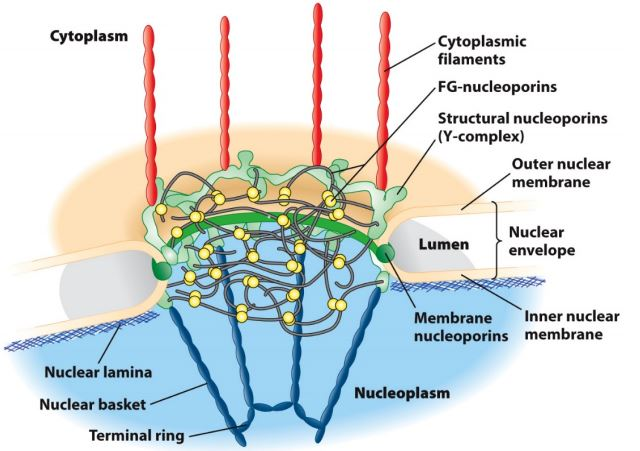
\includegraphics[width=0.7\textwidth]{images/poroNucleare.JPG}
                \caption{\small Struttura di un poro nucleare}
                \label{fig:mesh1}
            \end{figure}
        
    \subsection{Importazione}
        \subsubsection{Nuclear Localization Signal}
            NLS sta per \textit{nuclear localization signal}. L'importazione di una proteina nel nucleo è segnata dalla presenza di una sequenza di AA particolare: 7 AA di cui prolina, lisina e arginina le più presenti, per questo motivo hanno una carica positiva. \\
            Questa sequenza sta generalmente in prossimità del C-terminale e \textbf{non} viene rimossa.
            
        \subsubsection{Processo importazione}
            I fattori coinvolti nell'importazione di proteine nel nucleo sono:
            \begin{itemize}
                \item un recettore di trasporto nucleare, l'\textit{importina}
                \item una RAN (GTPasi, \textit{RAs-related Nuclear protein}), associata a GTP diventa prona ad associazione con importina, associata a GDP non ha affinità
                \item GAP e GEF
            \end{itemize}
            L'importazione segue gli step:
            \begin{enumerate}
                \item L'importina riconosce la sequenza NLS
                \item Il complesso importina-proteina attraversa il NPC grazie alle caratteristiche chimiche dell'importina stessa
                \item RAN (può diffondere attraverso il NPC) si associa a un GTP grazie ad una GEF (pre-esistente nel nucleo) che favorisce l'associazione all'importina e promuove il rilascio del cargo.
                \item RAN-GTP associata ad importina attraversa NPC
                \item una GAP (nel citoplasma) idrolizza il GTP di RAN a GDP, quindi abbiamo la dissociazione tra RAN e l'importina.
            \end{enumerate}
            La GEF nel nucleo e la GAP nel citoplasma mediano l'attivazione e l'inattivazione di RAN (tramite inclusione di GTP o idrolisi a GDP) che entra ed esce dal nucleo per esportare importina, con il fine di poterla riutilizzare.\\
            Per ogni ciclo di RAN si consuma un GTP.
            \begin{figure}[h]
                \centering
                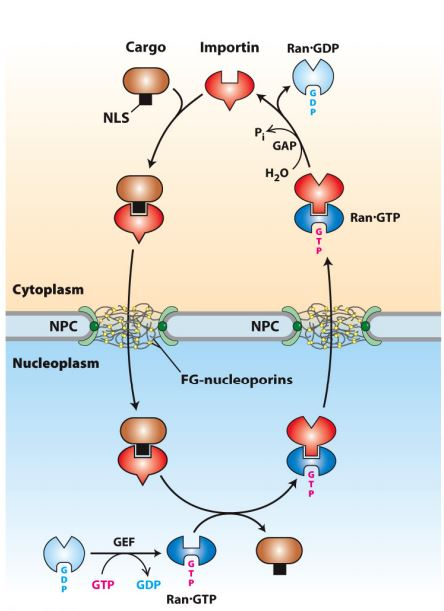
\includegraphics[width=0.5\textwidth]{images/import-exportNucleo.JPG}
                \caption{\small Molecole coinvolte nell'importazione del cargo e nell'esportazione dell'importina con il fine di compiere il ciclo nuovamente}
                \label{fig:mesh1}
            \end{figure}
            
    \subsection{Esportazione}
        \subsubsection{Nuclear Export Sequence}
            NES sta per \textit{nuclear export sequence} ed è una sequenza ricca di leucina (e un percentuali minori isoleucina, valina, metionina e fenialanina).
            
        \subsubsection{Processo esportazione}
            L'esportazione dal nucleo avviene per proteine che veicolano l'uscita di molecole sintetizzate nel nucleo, quali tRNA, mRNA o subunità ribosomiali.\\
            Per l'esportazione dal nucleo sono coinvolte proteine in grado di compiere \textit{shuttling}, ovvero hanno sia una sequenza NLS che NES per essere esportate e importate dopo aver compiuto il loro dovere, tra le quali \textit{exportin1} o \textit{CRM1}.
            \begin{enumerate}
                \item la proteina target espone il NES
                \item la sequenza NES viene associata a exportin1 o CRM1 (nel nucleo)
                \item avviene l'associazione a una RAN-GTP: la formazione del complesso per il trasporto è ora pronto.
                \item attraversamento NPC
                \item GAP promuove idrolisi di GTP di RAN-GTP che rilascia l'esportina, la quale rilascia il cargo.
            \end{enumerate}
            \begin{figure}[h]
                \centering
                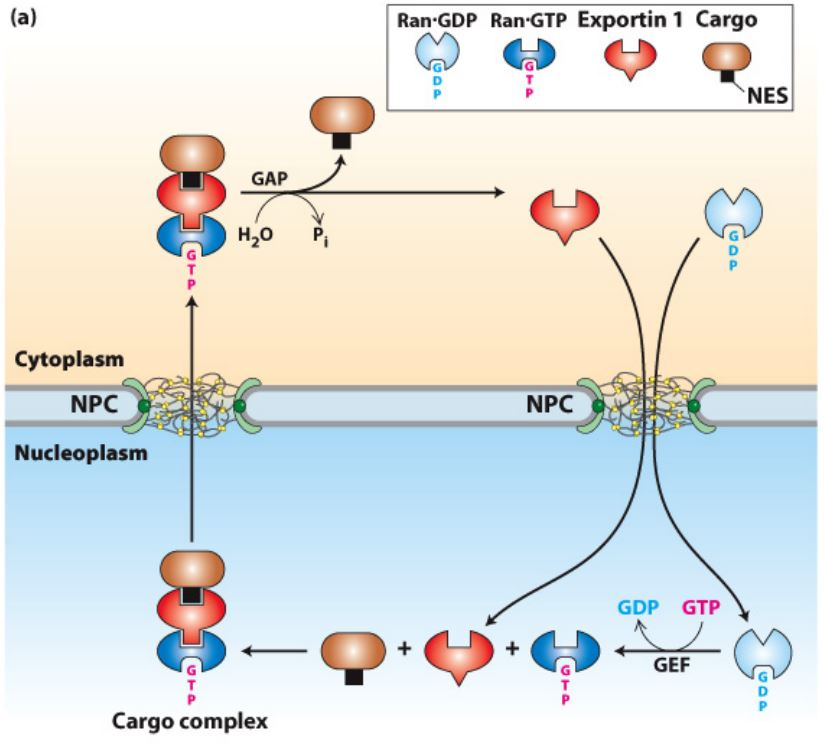
\includegraphics[width=0.5\textwidth]{images/exportNucleo.JPG}
                \caption{\small Molecole coinvolte nell'esportazione}
                \label{fig:mesh1}
            \end{figure}
            
            \textbf{RAN}\\
                RAN, oltre ad avere importanti compiti circa l'import e l'export dal nucleo, assume altri comportamenti in fasi cellulari diverse.\\
                Durante l'interfase protegge la comatina, mentre durante la mitosi fornisce le "coordinate" ai MT per la formazione del fuso mitotico utilizzando GEF e GAP, in prossimità della cromatina infatti c'è una concentrazione maggiore di RAN-GTP.
                
        \subsubsection{Esportazione attiva di mRNA}
            L'mRNA è trascritto nel nucleo e deve essere esportato per essere tradotto.\\
            La sua esportazione è associata a delle RNA binding protein (in particolare NXF1 e NXT1) che hanno propensione ad attraversare la maglia di nucleoporine FG e vengono dissociate dall'mRNA da un RNA-elicasi. 
            L'mRNA, NXF1 e NXT1 sono a questo punto liberi, e l'mRNA si può l'associare ai ribosomi.\\
            Le RNA binging protein possiedono una sequenza NLS che consente loro di essere importate nel nucleo per svolgere nuovamente la loro funzione (shuttling).
            \begin{figure}[h]
                \centering
                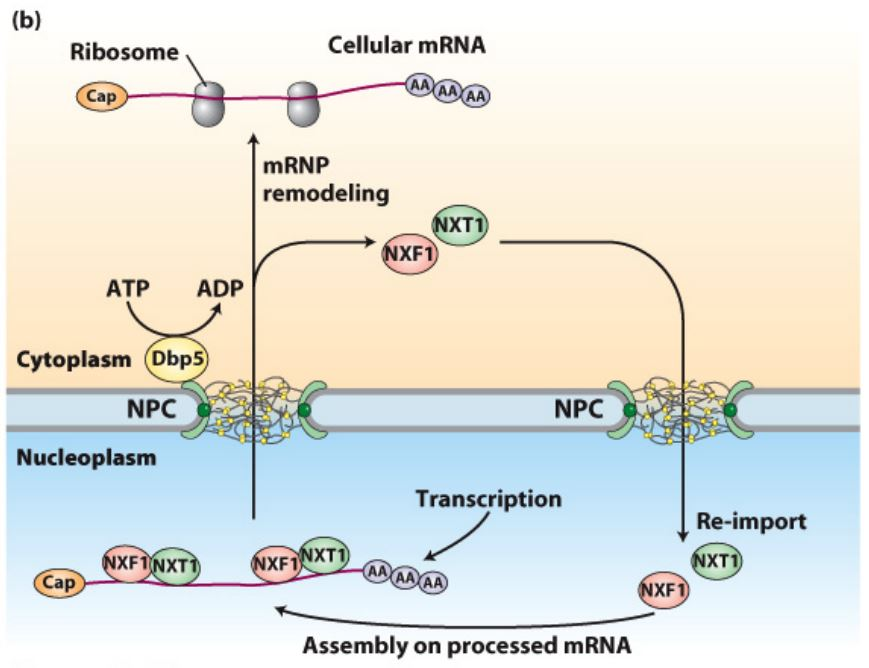
\includegraphics[width=0.5\textwidth]{images/exportNucleomRNA.JPG}
                \caption{\small Molecole coinvolte nell'esportazione si una molecola di mRNA maturo}
                \label{fig:mesh1}
            \end{figure}
    
\section{Destinazione: Mitocondrio}
    Il mitocondrio è un organello cellulare ottenuto dalle cellule eucariotiche per incorporazione di un altro organismo (vedi teoria endosimbiontica). 
    \subsection{Struttura mitocondrio}
        Il mitocondrio è composto da due membrane, la porzione completamente interna è chiamata matrice mitocondriale, lo spazio tra le due viene chiamato spazio intermembrana.\\
        Si occupa della respirazione cellulare e sulla sua membrana sono presenti le proteine che rendono possibile di questo processo. Racchiude il proprio genoma mitocondriale (DNA-M), le proprie RNA-P e tRNA. I complessi proteici codificati dal DNA-M sono composti in maggior parte da porzioni codificate dal DNA-C (cellulare): è pertanto necessario un coordinamento tra i geni del DNA-M e del DNA-C.
        In particolare le proteine sintetizzate nel citoplasma dal DNA-C devono raggiungere il mitocondrio.
        
    \subsection{Mitocondrial Targeting Sequence}
        Per MTS (mitocondrial targeting sequence), si intende una sequenza specifica posta all'N-terminale rappresentata da un $\alpha$E anfipatica di lunghezza variabile. 
        Dopo l'importazione, MTS viene rimossa.
        
    \subsection{Importazione}
        L'importazione nel mitocondrio avviene a livello post-traduzionale con la proteina non conformata tridimensionalmente.\\
        Sono coinvolte le seguenti molecole:
        \begin{itemize}
            \item HSP70: uno chaperon contro il ripiegamento
            \item TOM20 e TOM22: \textit{Traslocone of Outer Mitocondryal membrane} che non coinvolgono GTP
            \item TOM40: un poro generale della membrana esterna
            \item TIM44: \textit{Trascolone of Inner Mitocondryal membrane}
        \end{itemize}
        L'importazione nella matrice mitocondriale avviene secondo i seguenti step:
        \begin{enumerate}
            \item HSP70 riconosce MTS e impedisce alla proteina di ripiegarsi. Per questa operazione viene consumato ATP
            \item TOM20 e TOM22 predispongono la proteina all'importazione esponendo la MTS
            \item TIM44 si allinea a TOM40 spazialmente, per permettere alla proteina di attraversare entrambe le membrane simultaneamente
            \item HSP70 idrolizza ATP per permettere la traslocazione della proteina senza che avvenga un ripiegamento. Perchè avvenga la traslocazione è necessaria la differenza di gradiente protonico tra i lati della membrana.
            \item rimozione della MTS
        \end{enumerate}
        \begin{figure}[h]
            \centering
            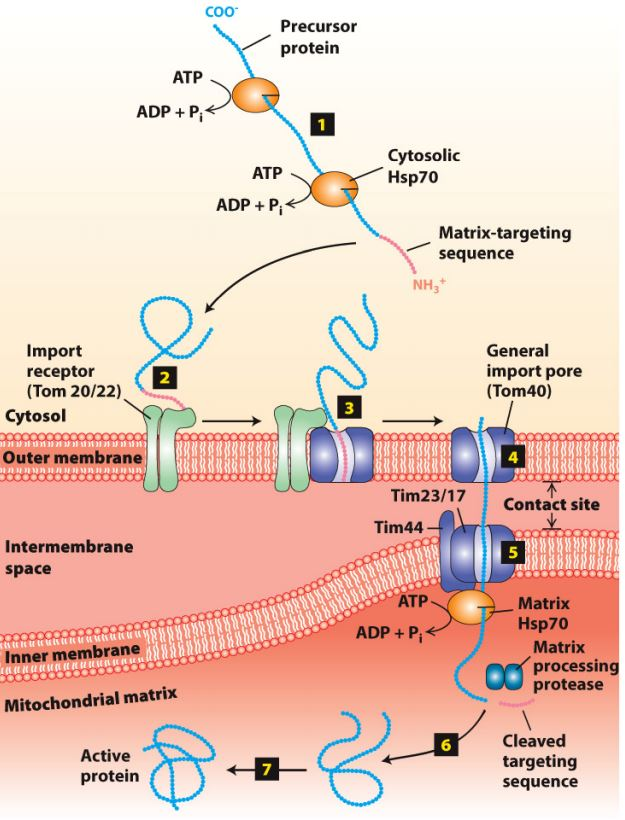
\includegraphics[width=0.7\textwidth]{images/importMito.JPG}
            \caption{\small Molecole coinvolte nell'importazione di una proteina svolta nella matrice mitocondriale}
            \label{fig:mesh1}
        \end{figure}
        
        \subsubsection{Destinazioni nel mitocondrio}
            Essendo un complesso formato da diverse membrane, proteine diverse avranno luoghi interni al mitocondrio differenti. In base alla loro destinazione si evidenzia una sequenza variabile adiacente a MTS.\\
            
            \textbf{Matrice mitocondriale}\\
                Presenta una MTS all'N-terminale, è il procedimento descritto in precedenza.\\
                
            \textbf{Integrali di membrana interna}\\
                Esistono diverse possibilità: 
                \begin{itemize}
                    \item Sequenza MTS all'N-terminale seguita da sequenza topogenica STA che permette l'inserzione nella membrana
                    \item Sequenza MTS all'N-terminale seguite da sequenze riconosciute da OXA1 (a livello della membrana interna, riconosce proteine nella matrice trasferite completamente e le reinseriscono nella membrana).
                    \item Sequenza primaria a-tipica, senza sequenza MTS all'N-terminale, ma con sequenze interne riconosciute da un recettore dedicato TIM. Dopo passaggio attraverso TOM40 c'è un interazione con un complesso TIM dedicato che inserisce la proteina nella membrana.
                \end{itemize}
            
            \textbf{Integrali di membrana esterna}\\
                Riguarda per lo più proteine che assumono la conformazione di barile$\beta$. Avviene grazie alla sequenza MTS all'N-terminale insieme a STA che consentono la diffusione interna al doppio strato lipidico. (TOM40 importa se stesso)\\
            
            \textbf{Spazio intermembrana}\\
                Esitono diverse sequenze che permettono l'arrivo di una proteina nella porzione inetrmembrana:
                \begin{itemize}
                    \item presenza MTS all'N-terminale (passaggio per TOM e successivamente TIM) con sequenza STA. Rilascio della proteina nella membrana interna, intervento di una proteasi che elimina la sequenza transmembrana per liberare la sequenza di AA nello spazio intermembrana.
                    \item presenza di MTS all'N-terminale specifica per il poro generale TOM40. Avviene una semplice diffusione, TIM44 non si allinea. La formazione di ponti disolfuro garantisce l'unidirezionalità del movimento. 
                \end{itemize}
            
\section{Destinazione: Cloroplasto}
    L'incorporazione del cloroplasto nelle cellule vegetali è associata alla stessa teoria endosimbiontica per i mitocondri. Le proteine che lo compongono sono per lo più codificate a livello di DNA-C.
    \subsection{Struttura cloroplasto}
        Il cloroplasto ha un'organizzazione più complessa del mitocondrio: sono sempre presenti le due membrame interna ed esterna, ma al posto della matrice si identifica lo stroma, all'interno del quale ci sono delle organizzazioni a cisterne chiamate tilacoidi.\\
        Solo a livello dei tilacoidi si nota il gradiente protonico citato in precedenza per i mitocondri. 
        
    \subsection{Importazione}
        L'importazione avviene attraverso step e componenti molto simili a quelle del mitocondrio. In particolare TOM diventano TOC (\textit{Traslocone of the Outer Chloroplast membrane}) e TIM diventano TIC (\textit{Traslocone of the Inner Chloroplast membrane}). \\
        La sequenza che determina l'importazione viene detta CTS, \textit{chloroplast transer sequence} che verrà tagliata dopo la traslocazione. CTS e MTS differiscono in larga parte. CTS è ricca di serine, treonine ma povera di acido glutammico e asparagina.\\
        La fonte energetica utilizzata per il trasferimento della proteina è l'ATP per prevenire il ripiegamento (sempre ad opera di HSP70). La proteina per poter transitare non deve essere ripiegata. Non c'è contributo del gradiente protonico per arrivare allo stroma (proprio perchè non c'è gradiente se non a livello dei tilacoidi). \\
        Nel caso una proteina debba raggiungere il tilacoide, esiste un'ulteriore sequenza segnale, riconosciuta da SRP che assieme a SRP receptor promuovono il trasferimento all'interno del tilacoide, successivamente la sequenza viene eliminata.
        Il tilacoide viene raggiunto tramite un canale diverso che permette di traslocare anche proteine non ripiegate. La fonte energetica per questo step è data dal gradiente protonico.

\section{Destinazione: Perossisomi}
    I perossisomi sono delle vescicole che sono adibiti a processare chimicamente delle molecole liberando $H_{2}O_{2}$. Dal momento che questa sostanza risulta tossica e dannosa, si confinano queste reazioni nei perossisomi. 
    I perossisomi sono generalmente sferici e contengono enzimi come l'\textit{ossidasi} e la \textit{catalasi}.\\
    Il metabolismo degli acidi grassi avviene a livello di mitocondrio e di perossisoma dando come risultato le stesse molecole ad eccezione per ATP, NADH e FADH$_{2}$, ma il perossisoma sono produce calore.\\
    L'ingresso della proteina nel perossisoma avviene a livello \textbf{post} traduzionale.
    
    \subsection{Peroxisome Targeting Sequence}
        Ci sono due tipologie di sequenze di targeting per il perossisoma che \textbf{non} venengono rimosse dopo l'importo. 
        La sequenza è \textit{serina-lisina-leucina}. Possiamo differenziare in:
        \begin{itemize}
            \item \textbf{PTS1}: la maggioranza, posta al C-terminale 
            \item \textbf{PTS2}: la minoranza, posta all'N-terminale
        \end{itemize}
        
    \subsection{Importazione}
        L'importazione di una proteina all'interno del perossisoma coinvolge i seguenti elementi:
        \begin{itemize}
            \item PEX5: un recettore sulla membrana citosolica del perossisoma per le PTS
            \item PEX14: proteina integrale di membrana per il trasporto
            \item PEX 10, 2, 12 integrali di membrana per ubiquitinazione
            \item PEX 1, 6, delle AAA ATPasi 
        \end{itemize}
        Questo processo prosegue secondo le fasi (in questo esempio la proteina possiede PTS1):
        \begin{enumerate}
            \item proteina viene interamente tradotta
            \item proteina espone PTS1 e viene riconosciuta dalla tasca dedicata di PEX5
            \item PEX5 interagisce con PEX14 che promuove la traslocazione nel lumen
            \item dissociazione PEX5 dalla proteina. Fino a questo punto non c'è dispendio di energia
            \item Dispendio ATP da parte di PEX 10, 2, 12 che mono-ubiquitinano PEX5
            \item PEX 1, 6 estraggono PEX5 dalla membrana che è libera di compiere di nuovo il suo dovere consumando ATP.
        \end{enumerate}
        Mutazioni distinte delle proteine della famiglia PEX (presenti in pazienti affetti dalla sindrome di Zellveger) hanno permesso di studiare a fondo il fenotipo dei perossisomi.\\
        Ad esempio, mutando PEX12, si assiste alla formazione di perossisomi che però rimangono privi di contenuto. La mutazione di PEX3 invece si manifesta con l'assenza dei perossisomi stessi. 
        \begin{figure}[h]
            \centering
            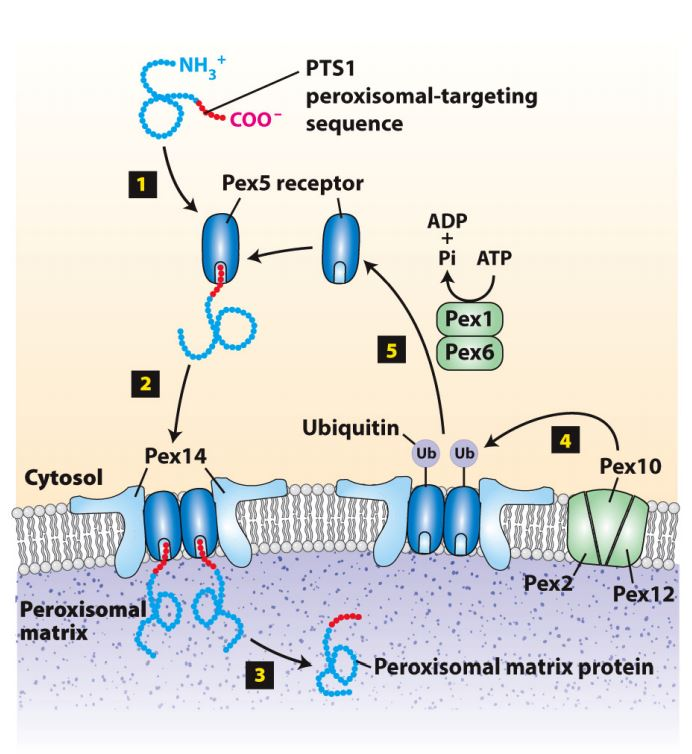
\includegraphics[width=0.5\textwidth]{images/importPerossisoma.JPG}
            \caption{\small Molecole coinvolte nell'importazione di una proteina nel perossisoma}
            \label{fig:mesh1}
        \end{figure}
        
    \subsection{Origine dei perossisomi}
        I perossisomi possono essere generati a partire da perossisomi pre-esistenti (grazie a PEX11) oppure ex-novo per gemmazione di una vescicola del RE. Nel secondo processo concorrono molte proteine della famiglia PEX e PMP70. \\

\section{Maturazione delle proteine}
    Per maturazione delle proteine si intendono eventi che possono avvenire a livello post o co-trazuzionale, vengono trasportate con SEC e avvengono nel RE o nel Golgi.
    
    \subsection{Glicosilazione}
        Per glicosilazione si intende l'aggiunta di componenti saccaridiche alla struttura proteica. Sono modifiche post-traduzionali che avvengono su AA specifici, ovvero serina e treonina (in corrispondenza di un OH nel lumen del Golgi) e asparagina (su un $NH_{2}$ nel lumen de RE).  \\
        La glicosilazione nel RE (\textit{N-linked glycosylation}) avviene seguendo gli step:
        \begin{enumerate}
            \item formazione del precursore con zuccheri (14 monomeri) assemblati covalentemente per la formazione del \textit{dolicolofosfato}, il precursore della glicosilazione vera e propria (associato ad asparagina)
            \item in presenza della sequenza segnale asparagina-x-serina/treonina avviene una glicosilazione a livello cotraduzionale degli N-terminali
        \end{enumerate}
        Alcuni step sono reversibili.\\
        La glicosilazione è necessaria al ripiegamento. La modifica degli zuccheri indicano infatti il corretto ripiegamento o servono alla recluta di chaperon per arrivare ad una conformazione corretta. Questa modifica è anche utile per la segnalazione della degradazione del polipeptide tramite l'albero saccaridico. 
        \begin{figure}[h]
            \centering
            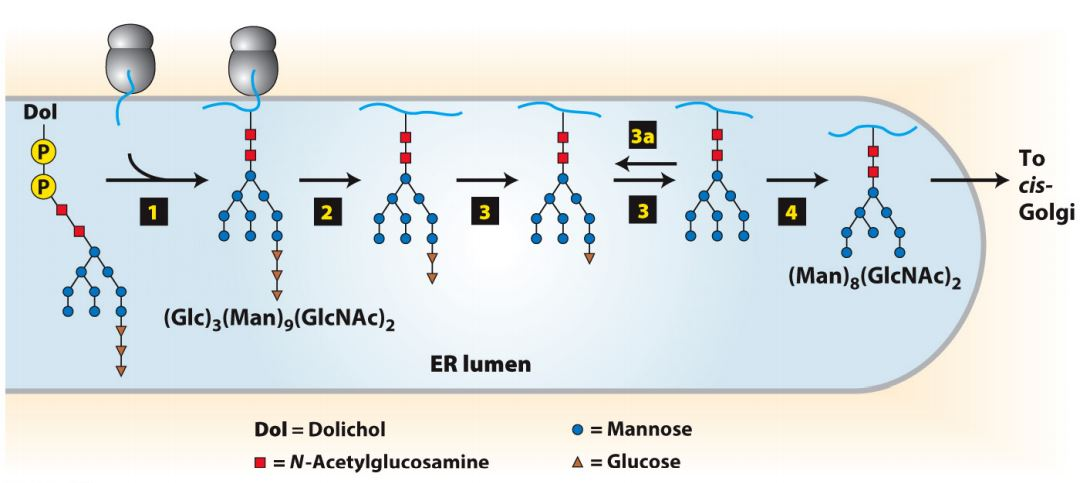
\includegraphics[width=0.7\textwidth]{images/glicosilazine.JPG}
            \caption{\small Glicosilazione di una proteina}
            \label{fig:mesh1}
        \end{figure}
        
    \subsection{Ponti disolfuro}
        I ponti disolfuro sono legami tra catene tra residui AA di cisteine che vengono effettuate solo a livello del lumen del RE.
        Viene mediato dall'enzima disolfuro-isomerasi (PDI) che contiene cisteine e un ponte disolfuro. \\
        La reazione è composta da due REDOX :
        \begin{enumerate}
            \item avviene una reazione tra PDI e una cisteina della proteina target che produce il ponte disolfuro
            \item avviene una reazione tra due cisteine del peptide target rilasciando PDI (grazie a potere dell'ossidazione) e spostando il ponte disolfuro tra i due residui AA
        \end{enumerate}
        La PDI può promuovere anche la rilocazione del ponte disolfuro.\\

        \begin{figure}[h]
            \centering
            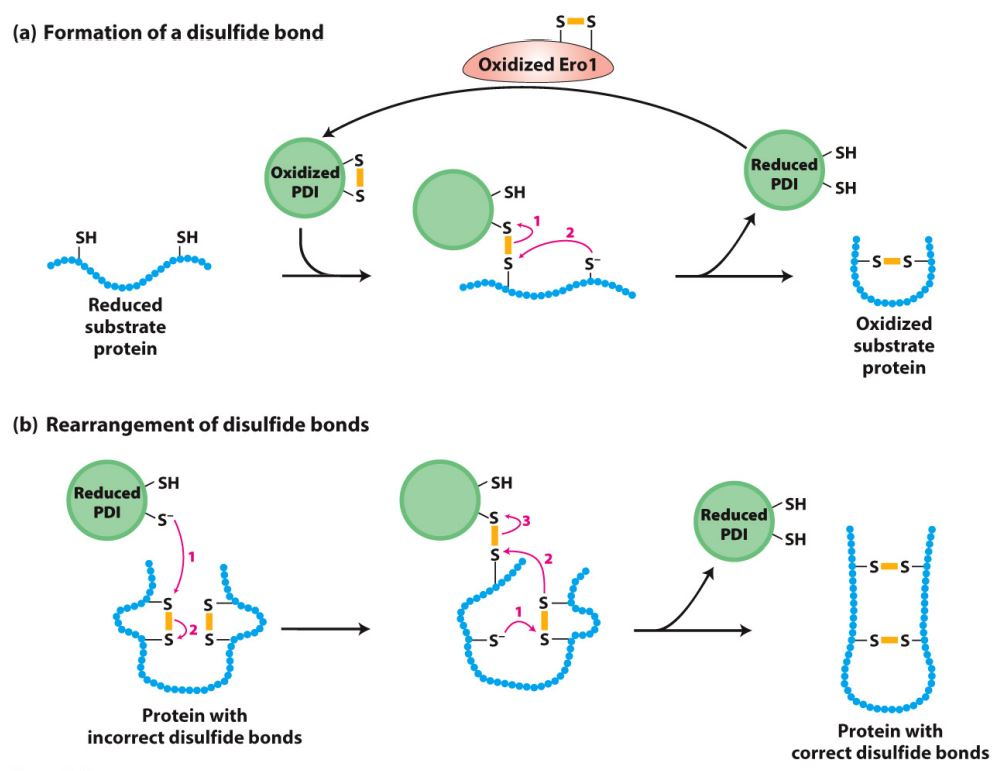
\includegraphics[width=0.6\textwidth]{images/pontiDisolfuro.JPG}
            \caption{\small Formazione dei ponti disolfuro e rilocazione attraverso PDI}
            \label{fig:mesh1}
        \end{figure}
        
    \subsection{Folding e assemblaggio di complessi multiproteici}
        Il folding e l'assemblaggio sono eventi che si verificano nel lumen del RE. 
        \subsubsection{Emoagglutinina del virus influenzale (HA)}
            Prendiamo come esempio il processo di assemblaggio della proteina che funge da antigene sul capside del virus influenzale. 
            \begin{enumerate}
                \item la proteina HA possiede una seguenza target all'N-terminale che permette l'accesso al RE. 
                \item avviene una glicosilazione cotraduzionale per ogni sequenza utile transitata: quest'operazione è utile al processo di folding che verrà effettuato dallo chaperon BiP.
                \item PDI forma dei ponti disolfuro
                \item la proteina di associa con altre proteine (calnexina e calreticolina) che legano specifici gruppi funzionali degli zuccheri, in questo modo la proteina viene ritenuta dal RE e non passerà attraverso il Golgi
                \item in corrispondenza della sequenza STA (Stop Tranfer Anchor) la proteina viene rilasciata nella membrana lipidica 
                \item la proteina funzionale è composta da un trimero, per questo motivo avverrà un riassemblaggio strutturale 
                \item proteolisi per la formazione di HA matura e fuoriuscita dal RE
            \end{enumerate}
                \begin{figure}[h]
                \centering
                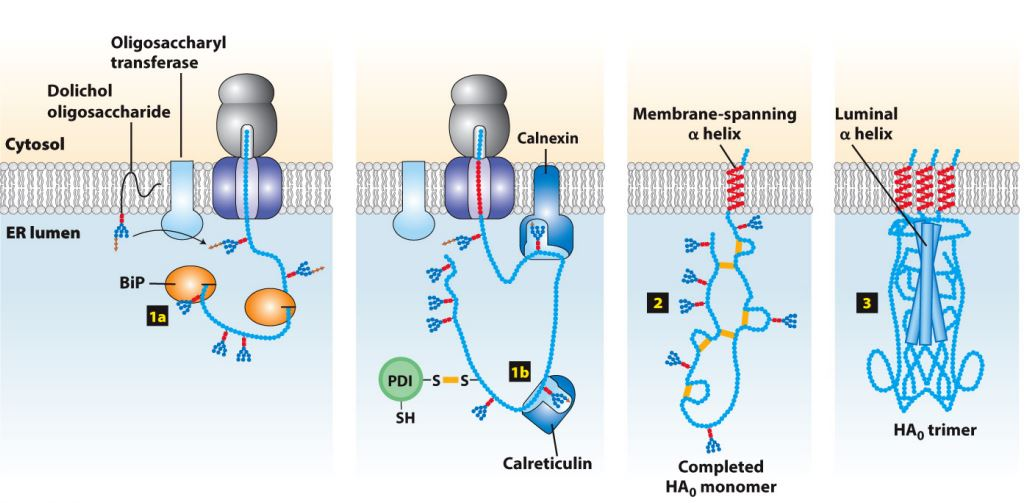
\includegraphics[width=0.7\textwidth]{images/ripiegamentoHA.JPG}
                \caption{\small Ripiegamento dell'emoagglutinina}
                \label{fig:mesh1}
            \end{figure}
        
        
        \subsubsection{Isomerizzazione della prolina}
            I carboni attorno ai legami peptidici assumono solamente dei determinati angoli, alcuni dei quali sono incompatibili con la formazione di strutture tridimensionali corrette (incompatibili con la formazione di determinate strutture secondarie). 
            Per questo motivo intervengono delle cis-trans-isomerasi (abbondanti nel lumen del RE) che catalizzano lo scambio conformazionale tra isomeri cis e trans.
        
        \subsubsection{Proteine mal-ripiegate}
            Le proteine non ripiegate correttamente non vengono rilevate come mature, per questo motivo non possono lasciare il RE e si crea un accumulo di materiale. L'accumulo causa a sua volta stress signaling.\\
            Esistono diversi metodi per controllare il corretto ripiegamento delle proteine, tramite quello che si chiama \textit{unfolded protein response} (UPR) tra cui il comportamento di Ire1.
            \begin{enumerate}
                \item Lo chaperon BiP cerca di ripiegare correttamente le proteine. Quando non è impegnato in questo compito, BiP è associato alla proteina di membrana Ire1.
                Quando la concentrazione di BiP libera è altra, Ire1 non vi è associata e genera un segnale citoplasmatico tramite un mRNA per cui lo "splicing" non è completato (Hac1).
                \item Ire1 ad effettua le modifiche a questo mRNA per farlo maturare (attua un'attività nucleosidica su un introne anomalo)
                \item traduzione del mRNA per ottenere altri chaperon BiP.
            \end{enumerate}
            Ire1 assume anche altri compiti, per esempio la sua alterata espressione genica collabora al signaling per la morte cellulare, infatti fa maturare miRNA per la regolazione della traduzione del gene pro-apoptotico.\\
            La situazione di stress signaling prodotta dall'accumulo di proteine malripiegate è spesso utilizzata sperimentalmente utilizzando la tunicamicina (un antibiotico che blocca le modifiche all'ancora lipidica necessaria al processo di glicosilazione).\\
            
    \subsection{Degradazione proreica}
    \begin{figure}[h]
            \centering
            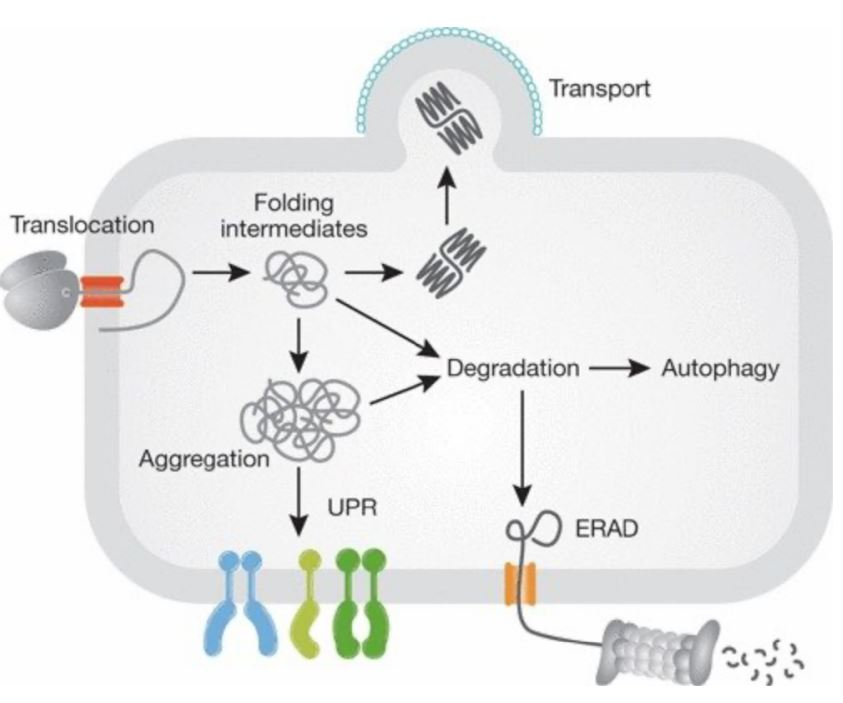
\includegraphics[width=0.5\textwidth]{images/degradazione.JPG}
            \caption{\small Diversi destini per proteine ripiegate e mal-ripiegate}
            \label{fig:mesh1}
        \end{figure}
        La degradazione delle proteine può avvenire tramite metodi che differiscono dall'utilizzo del proteasoma. Per l'operazione che si descrive ora si necessita della traslocazione dal lumen al citosol.\\
        L'enzima mannosidasi marca le proteine che necessitano di traslocazione nel citosol (dislocazione non per proteine glicosilate). Oltre alla mannosidasi esitono altri metodi per la traslocazione (di proteine glicosilate) che però non sono noti.\\
        Esiste un complesso chiamato ERAD (ER associated degradation), formato da 4 proteine integrali di membrana che insieme a p97 (AAA-ATPasi) strappa proteine destinata alla degradazione dalla membrana del RE. \\
        Se questo processo non va per il meglio si può attivare un UPR, altrimenti interviene ERAD fa passare le proteine nel citosol e contemporaneamente le poliubiquitina.
        

\pagebreak